\chapter{Results}

% Eine mögliche Struktur der Arbeit sieht wie folgt aus:

% \begin{enumerate}
%     \item \textbf{Einleitung}\\
%         In der \emph{kurzen} Einleitung wird die Motivation für die Arbeit
%         dargestellt und ein Einblick in die kommenden Kapitel gegeben.
%     \item \textbf{Theoretische Grundlagen}\\
%         Alles was an theoretischen Grundlagen benötigt wird, sollte auch eher kurz gehalten werden.
%         Statt Grundlagenwissen zu präsentieren, eher auf die entsprechenden Lehrbücher verweisen.
%         Etwa: Tiefer gehende Informationen zur klassischen Mechanik entnehmen Sie bitte \cite{kuypers}.
%     \item \textbf{Ergebnisse} \\
%         Der eigentliche Teil der Arbeit, das was getan wurde.
%     \item \textbf{Zusammenfassung und Ausblick} \\
%         Zusammenfassung der Ergebnisse, Optimierungsmöglichkeiten, mögliche weitergehende Untersuchungen.
% \end{enumerate}

% Die Gliederung sollte auf der einen Seite nicht zu fein sein, auf der anderen Seite
% sollten sich klar unterscheidende Abschnitte auch kenntlich gemacht werden.

% In der hier verwendeten \KOMAScript-Klasse \texttt{scrbook} ist die oberste Gliederungsebene,
% die in der Bachelorarbeit verwendet werden sollte, das \texttt{\textbackslash chapter}.

% Ein Kapitel sollte erst dann in tiefere Gliederungsebenen unterteilt werden, wenn es auch wirklich etwas zu unterteilen gibt. 
% Es sollte keine Kapitel mit nur einem Unterkapitel (\texttt{\textbackslash section}) geben.

% In dieser Vorlage ist die Tiefe des Inhaltsverzeichnisses auf \texttt{chapter} und \texttt{section} beschränkt. 
% Möchten Sie diese Beschränkung aufheben, entfernen Sie den Befehl
% \begin{verbatim}
%             \setcounter{tocdepth}{1}
% \end{verbatim}
% aus der Präambel oder ändern Sie den Zahlenwert entsprechend. Das Inhaltsverzeichnis sollte für eine Bachelorarbeit auf eine Seite passen.

\section{Analysis of the Fixed Rate Trigger}

The functionality of the FRT is described in section~\ref{sec:daq}. In the following section, the spectrum of the data aquired by the FRT will be analyzed in 
detail. In this section, an event will mean everyting that is measured within a single trigger window. A link to the exact data used can be found 
in the appendix. The following Plots give an overview of the charge distribution of the signals collected by the FRT. Firstly, the charge distribution making up a 
single event are shown in the Histograms~\ref{fig:single_charge_hist}. As expected, the counts follow a visible poisson distribution.

\begin{figure}
    \centering
    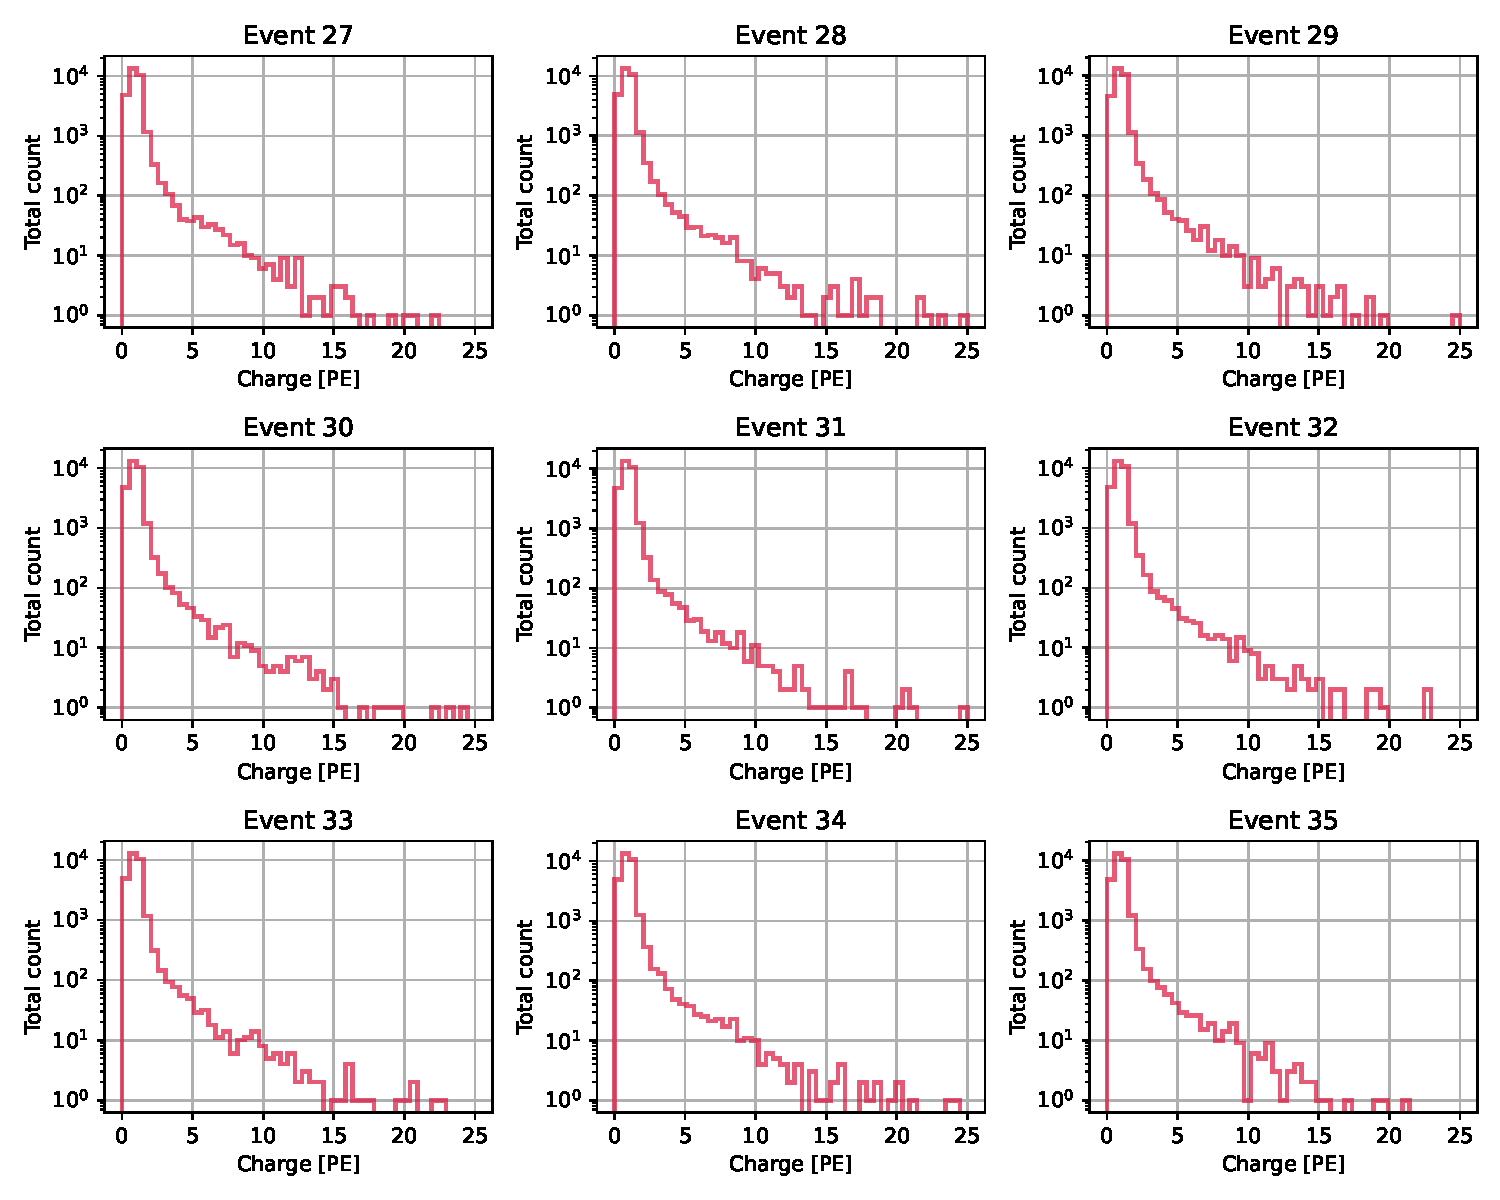
\includegraphics[width=0.7\textwidth]{Plots/single_charge_hist.pdf}
    \caption{histograms of the charge distribution of a subset of FRT events from April 2016.}
    \label{fig:single_charge_hist}
\end{figure}


In the histograms~\ref{fig:monthly_charge_hist} the data is grouped together in a way that shows one entry as one event where the charges are summed up, meaning the 
integrals of the histograms~\ref{fig:single_charge_hist} would each make up one event. 

\begin{figure}
    \centering
    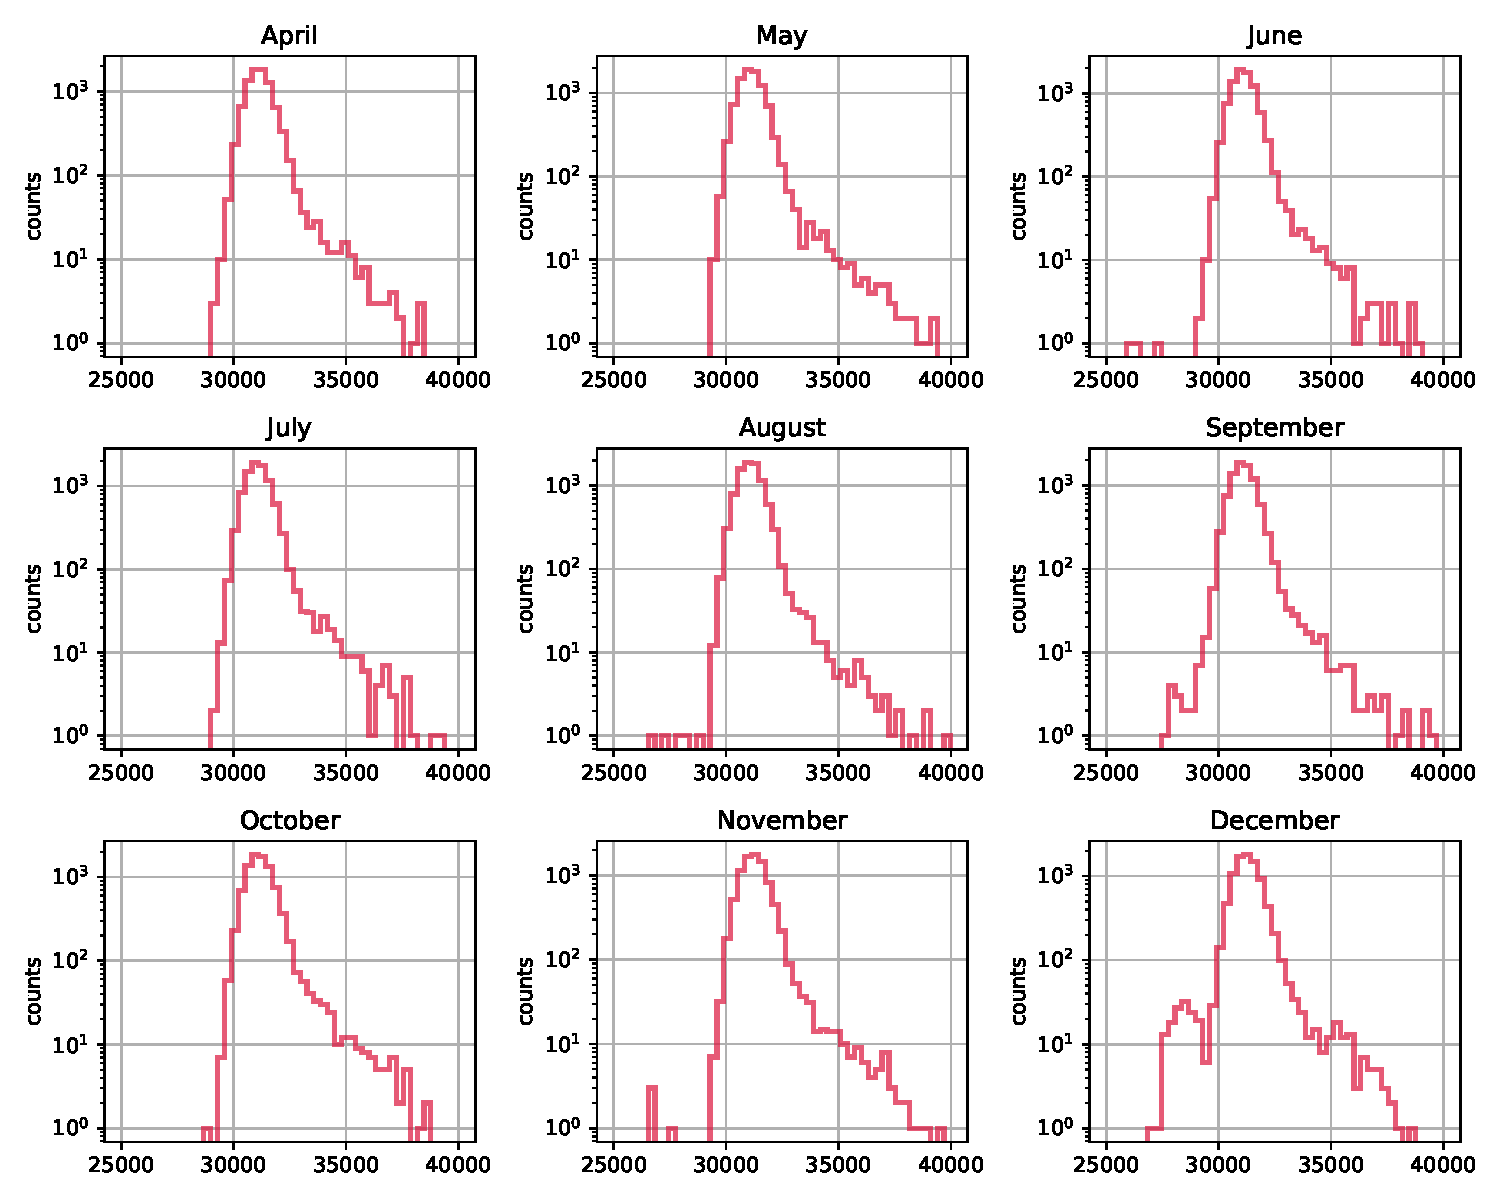
\includegraphics[width=0.7\textwidth]{Plots/monthly_charge_hist.pdf}
    \caption{histograms of the charge distribution of all events making up entire months of 2016.}
    \label{fig:monthly_charge_hist}
\end{figure}

Best visible in the histogram for may, up to a charge value of around \SI{3300}{PE} the count rate follows a pretty clear gaussian distribution, which is followed 
by an exponential decline. If the background noise, whatever it might be, follows a gaussian distribution, a sensible idea would be to fit a gauss for the charge 
values up to the critical point, after which the distribution type changes. Then a filter which is looking for 'real' events might filter out anything that lies 
within the fitted realm. 

\section{Muon Rate}

As explained in \ref{sec:coin} the probability function of coincidence events against total events can be estimated to follow a poisson distribution.
A theoretical distribution for different trigger windows is shown in figure(). In order to put this into a meaningful context, data() is analyzed to extract a 
connection between the event rate and other significant variable, such as energy. 

\section{Description of plots for later use}
\begin{figure}
    \centering
    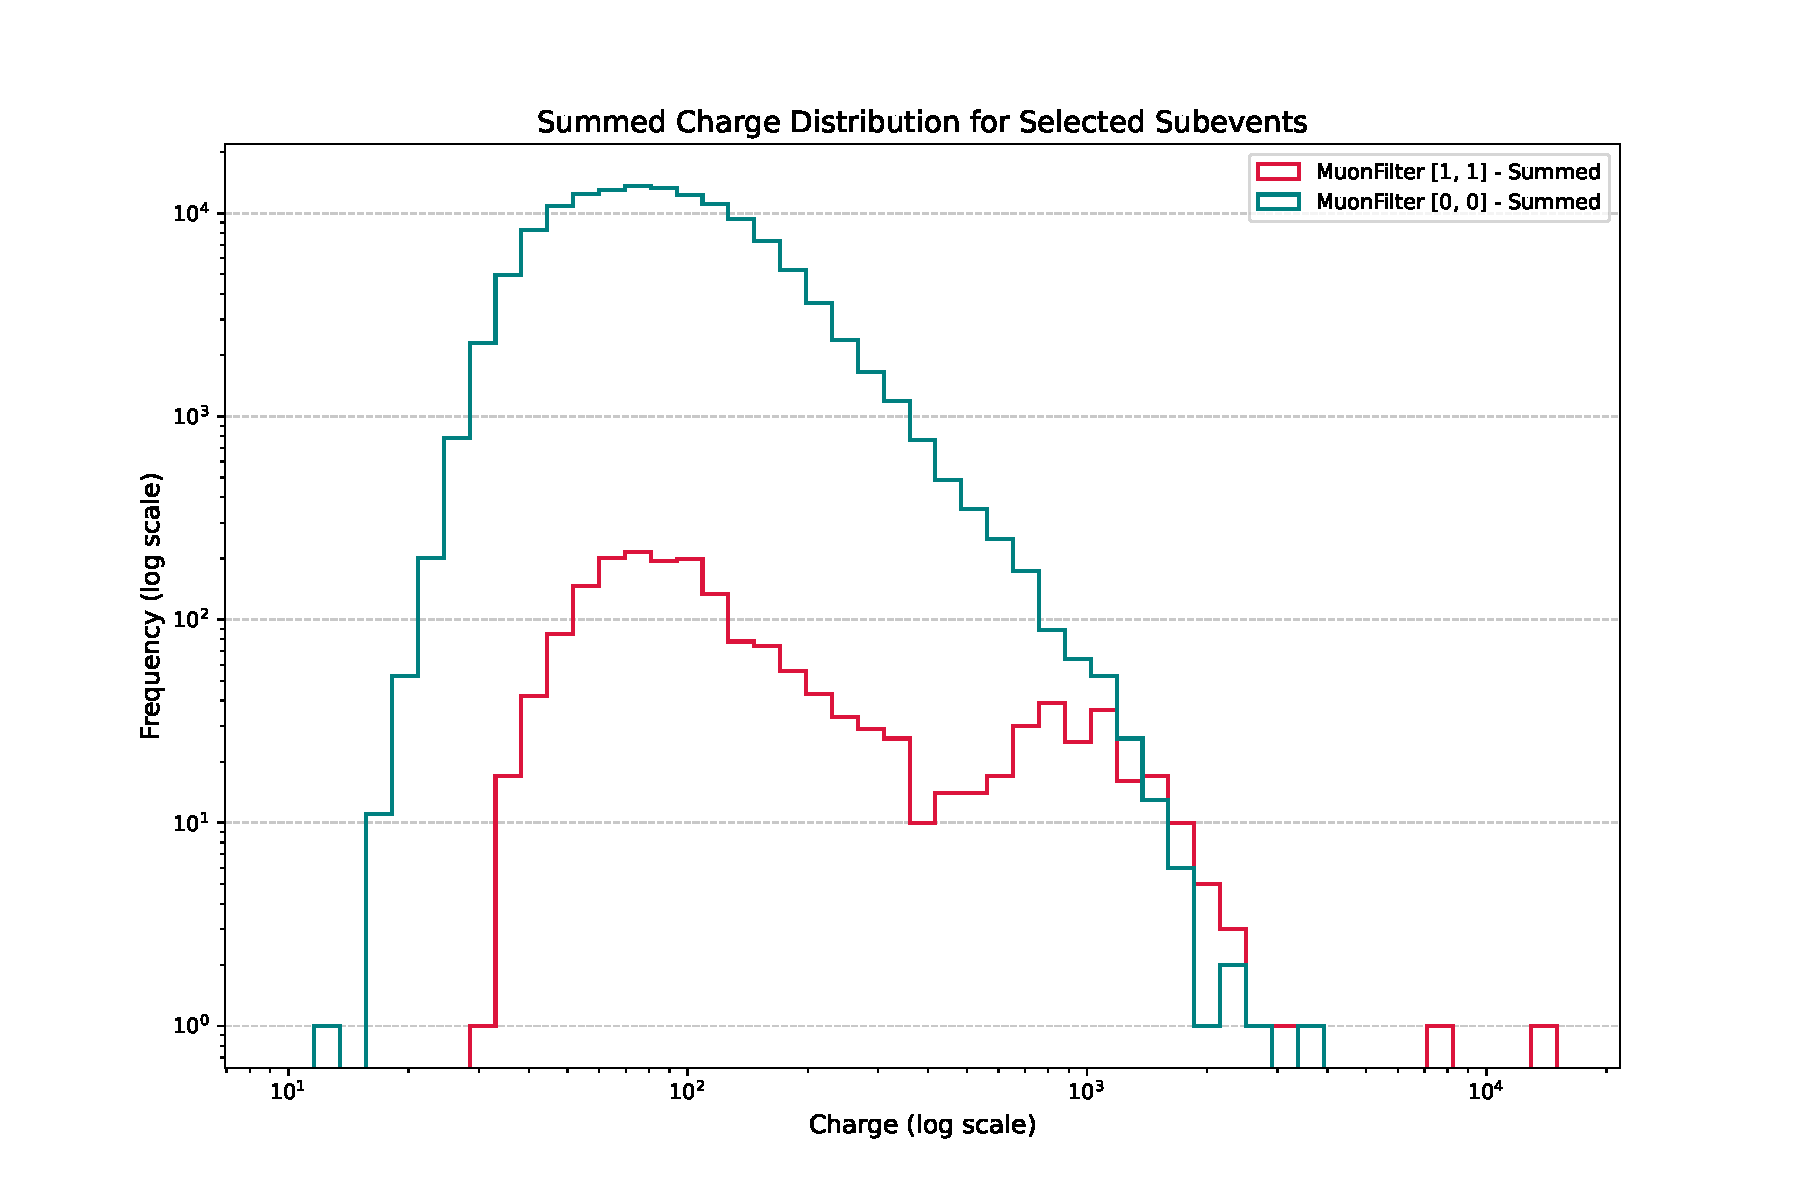
\includegraphics[width=0.7\textwidth]{Plots/frt_muon_filter_sub.pdf}
    \caption{histogram showing FRT-subevents which did and did not pass the muon filter.}
    \label{fig:frt_mu_sub}
\end{figure}

figure~\ref{fig:frt_mu_sub} shows the distribution of charges that the detector measures for each subevent. A subset of these subevents pass the muon filter, 
meaning they are most likely actual muon events. The expectation would be, that most of the subevent which pass the muon filter would be seen at higher charge values,
since their energy and therefore the intensity of Cherenkov radiation would be much greater that a signal caused by any kind of noise. As can be seen in the 
histogram however, this is not the case. Taking a look at the linear visiualization of the distributions, as done in figure~\ref{fig:frt_mu_sub_comp}, it is obvious that 
both spectrums are clearly poisson distributed with a peak at the same charge value of around 80 PE. While a poisson distribution can be expected, it is 
suspicious that the peak of both distributions are around the same value. 

\begin{figure}[H] % The [H] forces the figure to be placed exactly here
    \centering
    \begin{subfigure}{0.49\textwidth}
        \centering
        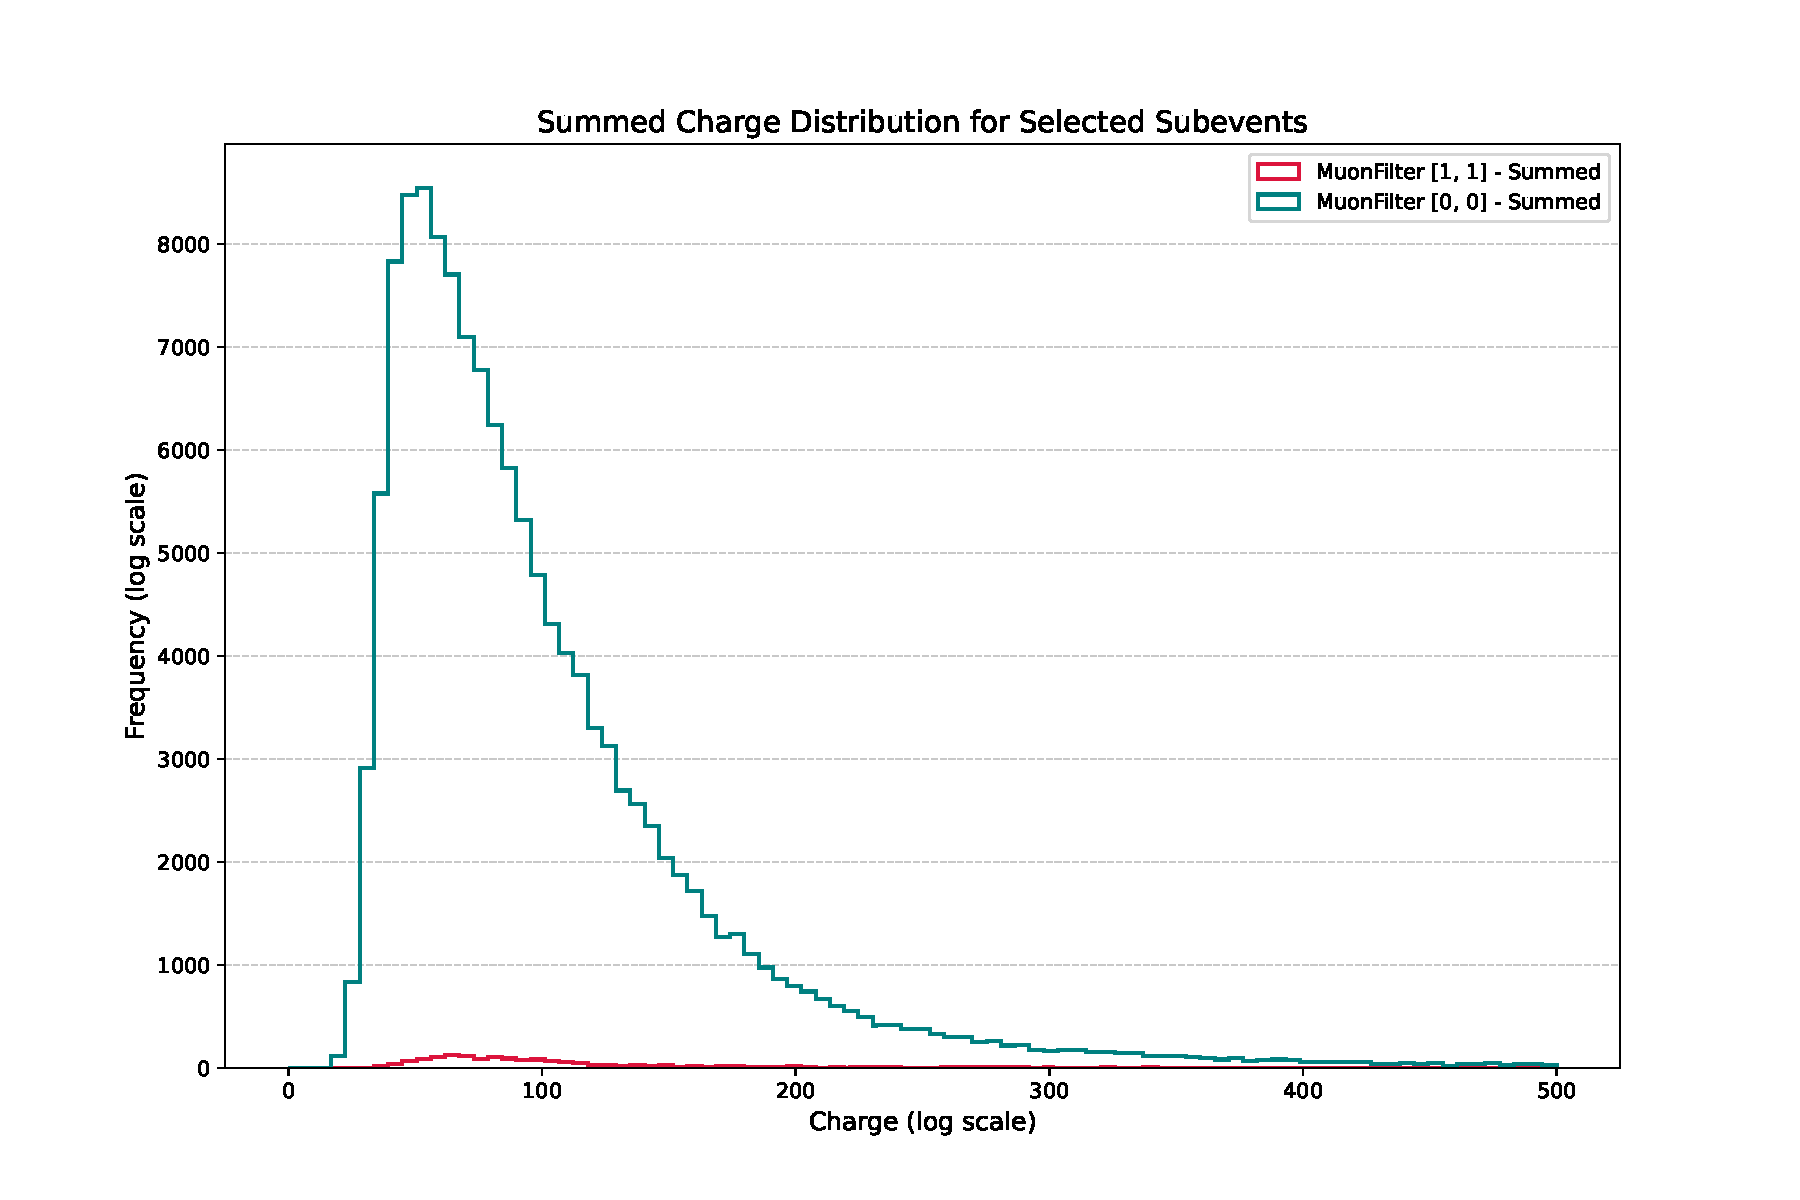
\includegraphics[width=\textwidth]{Plots/frt_muon_filter_sub_lin.pdf}
        \caption{Subfigure 1}
        \label{fig:sub1}
    \end{subfigure}
    \hfill % Adds spacing between the subfigures
    \begin{subfigure}{0.49\textwidth}
        \centering
        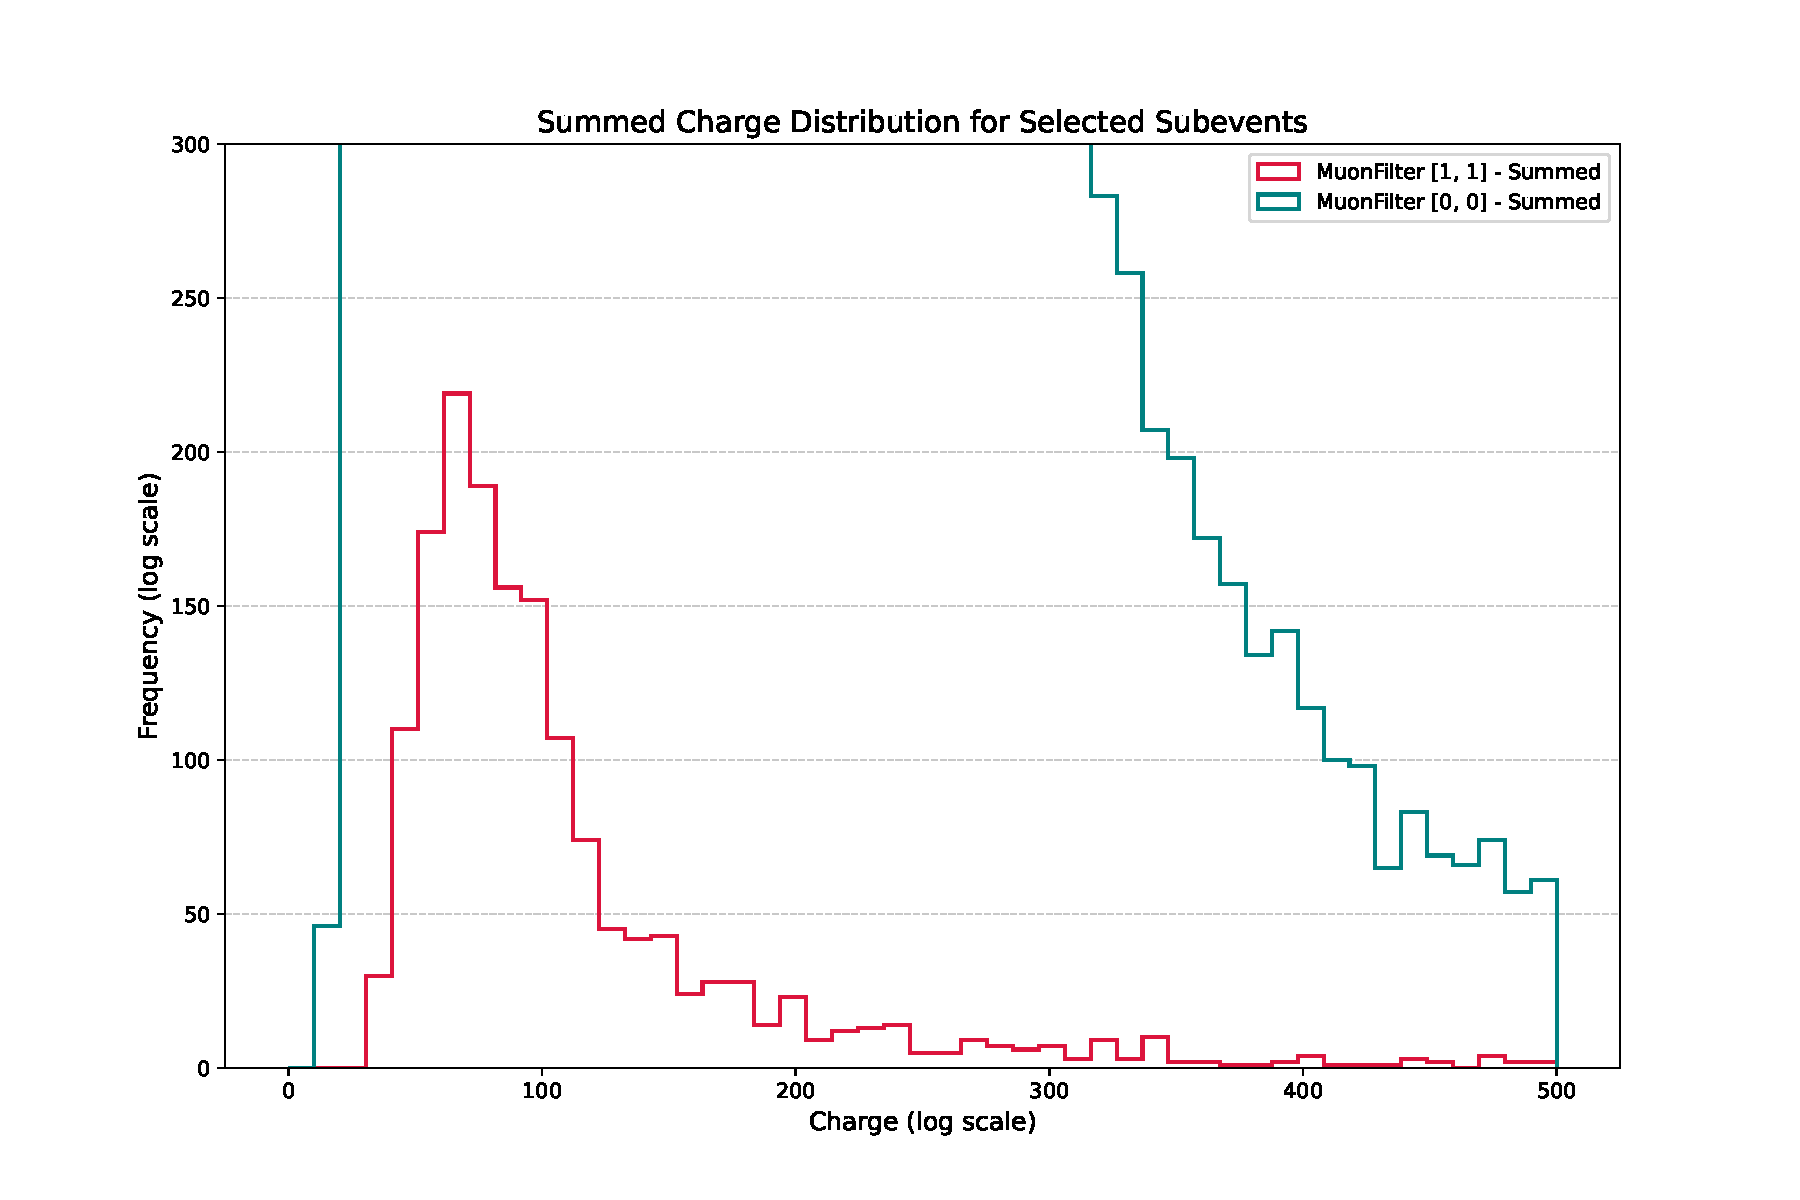
\includegraphics[width=\textwidth]{Plots/frt_muon_filter_sub_mod1.pdf}
        \caption{Subfigure 2}
        \label{fig:sub2}
    \end{subfigure}
    \caption{Main caption describing both plots.}
    \label{fig:frt_mu_sub_comp}
\end{figure}

Figure~\ref{fig:frt_mu_2} shows the spectrum of \num{5032} FRT events, aswell as the spectrum of a subset of those events, which passed the muon filter, categorizing 
them as muon events. The expectation here is that the muons event would have a charge distribution shifted to the right of the distribution making up the events 
that do not satisfy the muon filter. This is assuming that whatever does not pass the muon filter is mostly noise. Any kind of background is expected to consist
of signals carrying significantly less energy than the muons hitting the detector. Evendetly, this expectation is not fully satisfied by the histogram in 
figure~\ref{fig:frt_mu_2}. While at higher charge values, the muon events start to make up the majority of the counts, the counts in these regions do not make up 
a significant portion of the muon events themselves. Also, the peak of the muon events spectrum lies at around \num{2000}~PE, almost the same as the peak of the 
failed events. The majority of both event types lie within the same region of charge values, meaning that there is a significant overlap in their distribution, 
which makes a discrimination of muon event based solely on the charge measured by the detector, not directly possible. 
\begin{figure}
    \centering
    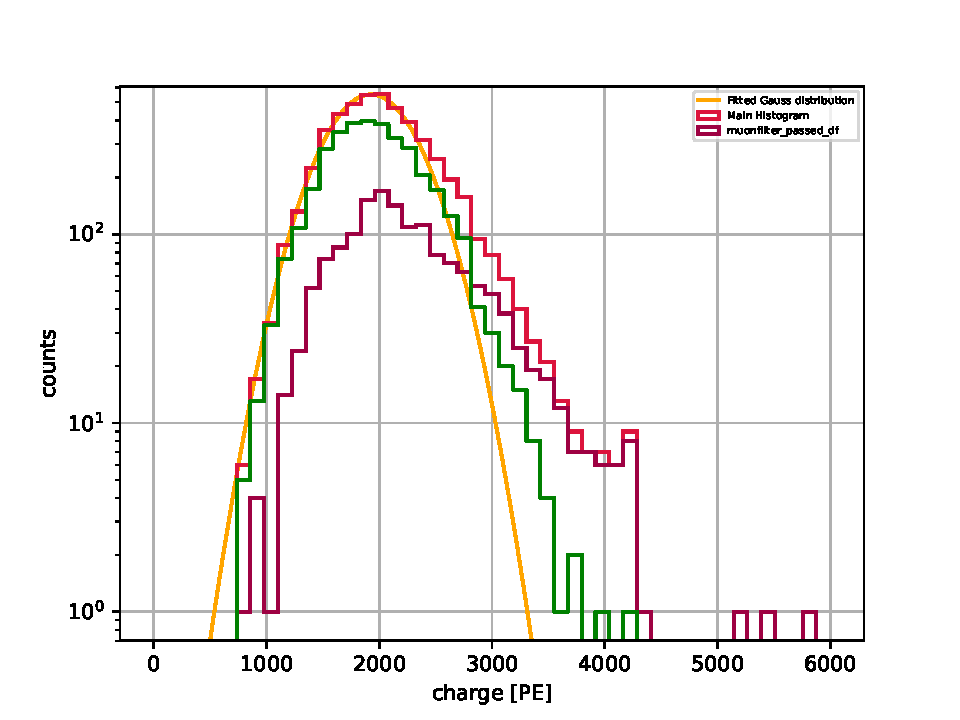
\includegraphics[width=0.7\textwidth]{Plots/frt_muon_filter.pdf}
    \caption{histogram showing FRT-events which did and did not pass the muon filter.}
    \label{fig:frt_mu_2}
\end{figure}


\section{coincidence probability}

Assuming the capability to detect coincident events by their signature in the DOMs, the question still arises, what exactly constitutes the coinciding event. As 
there seems to be a significant probability for an event leaving a signature similar to that of a muon, but not being one. In the following segment, an estimation
will be made on how likely it is for a coincident event to be a true coincident muon, based on different types of knowledge about the event. 